\subsection{Anforderungen der Erklärungen}
\label{sec:explanation_requirements}

Mithilfe der Rohanforderungen und Ziele aus dem Workshop sowie den erstellten Personas können sowohl funktionale als auch nicht-funktionale Anforderungen für Erklärungen in NUNAV entwickelt werden

\subsubsection{Nicht-Funktionale Anforderungen}

Als Methode zum Ableiten der konkreten NFRs wurde das Aufstellen eines Qualitätsmodells gewählt \cite{schneider2012abenteuer}. Das Modell ist in \autoref{fig:nunav_explanation_quality_model} dargestellt. Bei der Erstellung wurde iterativ Rücksprache mit den verschiedenen Teilnehmern des Workshops gehalten. Als Basis für die Qualitätsziele wurden die in dem Modell für Erklärungen unter \textit{Objectives} aufgeführten Ziele verwendet. Die Endfassung der Anforderungen wurde schlussendlich vom Teamleiter des \glqq Mobile Application\grqq{}-Teams abgesegenet.

Normalerweise findet eine systematisierte Anforderungserhebung, wie sie im Rahmen dieser Arbeit erfolgt ist, bei \textit{Graphmasters} keine Anwendung. Die Rolle des \textit{Requirements Engineers} hat sich daher als herausfordernd herausgestellt und ist in den agilen Prozessen von \textit{Graphmasters} nicht vorgesehen. Insbesondere fehlte zum Teil das Verständnis, warum vor allem Qualitätsanforderungen in der folgend vorgestellten, konkreten Weise vorliegen sollen. In den Rücksprachen wurde deutlich, dass Ziele für die Produkte normalerweise deutlich abstrakter gehalten werden. Für eine Evaluation der Integration von Erklärungen im Rahmen dieser Arbeit werden die konkreten Anforderungen zur Prüfung allerdings benötigt.

\begin{figure}[htb!]
    \centering
    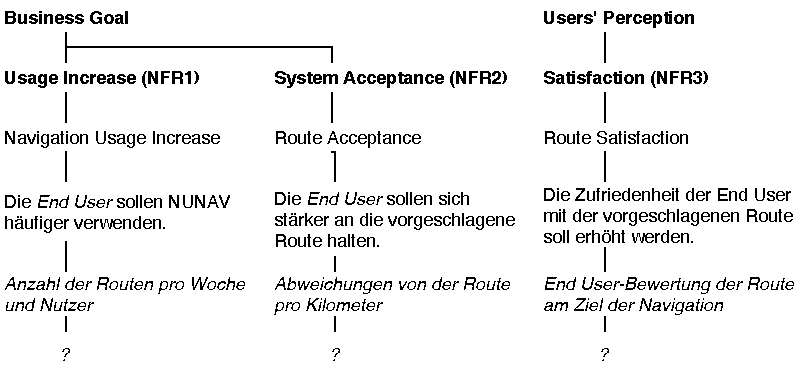
\includegraphics[width=\textwidth]{contents/06_model_evaluation/01_integration/res/quality_model.pdf}
    \caption{Qualitätsmodell für die Integration von Erklärungen in NUNAV Navigation}
    \label{fig:nunav_explanation_quality_model}
\end{figure}

In \autoref{fig:nunav_explanation_quality_model} ist zu erkennen, dass für \textit{Graphmasters} im Allgemeinen die Erhöhung der Nutzung und die Akzeptanz des Systems im Vordergrund stehen. Bei der Nutzung ist für \textit{Graphmasters} die interessanteste Metrik die Anzahl der aktiven Nutzer. Da sich eine Messung von Veränderungen dieser durch die Integration von Erklärungen allerdings nicht über einen kurzen Zeitraum messen lässt, wurde  als Metrik die Anzahl der Routen pro Nutzer und Woche vorgeschlagen und schließlich auch durch \textit{Graphmasters} bestätigt. Für die Akzeptanz des Systems ist ein Ziel, dass sich die \textit{End User} möglichst viel an die vorgeschlagene Route halten. Als Metrik wurde hierfür die Anzahl der Abweichungen von der Route pro Kilometer verwendet.

Ein weiteres wichtiges Ziel von \textit{Graphmasters} ist die Zufriedenheit der \textit{End User} mit den Routen. Hierfür bestand bereits vor dem Beginn dieser Arbeit eine Metrik. \textit{End User} können bei Erreichen des Ziels einer Navigation auf einer Skala mit ein bis fünf Sternen angeben, wie zufrieden sie insgesamt mit der Route waren. Bisher wurde diese Metrik allerdings noch nicht systematisch ausgewertet.

Für alle Metriken fällt auf, dass in \autoref{fig:nunav_explanation_quality_model} keine Sollwerte definiert sind. Aus den Gesprächen hat sich ergeben, dass für \textit{Graphmasters} erstens nicht wichtig ist, um wie viel die verschiedenen Metriken sich verbessern, solange mit der Integration von Erklärungen eine Besserung eintritt. Außerdem ist sind keine Basiswerte vorhanden, auf die man sich beziehen kann. Aus diesem Grund wurden die konkreten Anforderungen in Bezug auf signifikante Unterschiede formuliert. Die Formulierungen orientieren sich dabei an gängigen Vorlagen, enthalten allerdings nicht die in den Vorlagen geforderten Sollwerte \cite{rajnish2010quality, alexander2002writing}:

\begin{enumerate}
    \item [NFR1] Die Anzahl der gefahrenen Routen mit \textit{NUNAV Navigation} pro Nutzer und Woche soll signifikant messbar erhöht werden.
    \item [NFR2] Die durchschnittliche Anzahl der Abweichungen der Nutzer pro Kilometer von der durch \textit{NUNAV Navigation} vorgeschlagenen Route soll signifikant messbar verkleinert werden.
    \item [NFR3] Die durchschnittliche Bewertung der Route am Ende der Navigation in \textit{NUNAV Navigation} soll signifikant messbar erhöht werden.
\end{enumerate}

\subsubsection{Funktionale Anforderungen}

In diesem konkreten Fall stand die Integration von Erklärungen als Lösungsansatz zum Erreichen der Ziele bereits fest. Daher wurden die \textit{Explanation Goals} aus dem Modell für Erklärungen ausgewählt, welche in Erklärungen umgesetzt werden sollten. Dabei steht vor allem auch die Frage im Raum, welche Aspekte genau erklärt werden müssen \cite{kohl_explainability_2019}.

Ein Ergebnis des durchgeführten Workshops war die Verständnisprobleme der Nutzer, welche durch Erklärungen gelöst werden sollen und erste Umsetzungsideen. Aus diesen beiden Punkten konnten \textit{Transparency} und \textit{Scrutability} als Ziele für die Integration von Erklärungen abgeleitet werden.
% Da die vorherigen Qualitätsanforderungen sehr Allgemein auf \textit{NUNAV Navigation} bezogen sind, ist das Ziel, dass sich alle integrierten Erklärungen positiv auf die Qualitätsziele auswirken.

Auch die Konkretisierung der funktionalen Anforderungen ist iterativ erfolgt. Eine Herausforderung dabei war vor allem, dass \textit{Graphmasters} in der Regel keine konkreten Anforderungen formuliert, sondern direkt anhand von Ideen Mockups erstellt und dann iterativ mehrere Prototypen entwickelt.

Für die funktionalen Anforderungen wurde ein Zielbaum ähnlich zu Qualitätsmodellen aufgestellt, in dem die Konkretisierungsschritte zu sehen sind. \autoref{fig:nunav_explanation_functional_model} stellt diesen dar.

\begin{figure}[htb!]
    \centering
    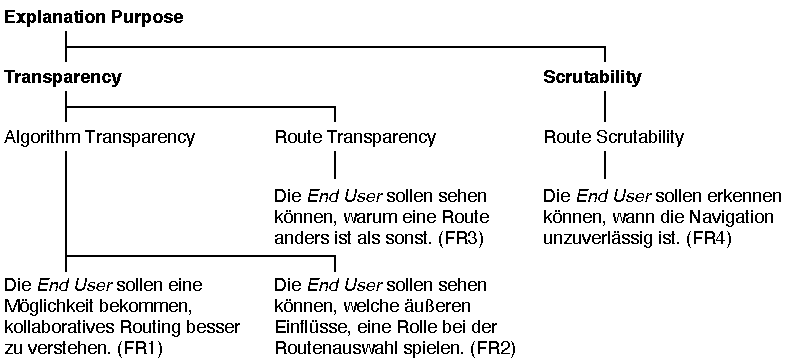
\includegraphics[]{contents/06_model_evaluation/01_integration/res/functional_model.pdf}
    \caption{Konkretisierungsschritte bei der Entwicklung der funktionalen Anforderungen an Erklärungen in \textit{NUNAV Navigation}}
    \label{fig:nunav_explanation_functional_model}
\end{figure}

\newpage

Aus den Konkretisierungsschritten (siehe \autoref{fig:nunav_explanation_functional_model}) wurden schlussendlich folgende funktionalen Anforderungen abgeleitet:
% . Die in der Abbildung als FR1 abgebildete unkonkrete Anforderung wurde im letzten Konkretisierungsschritt in zwei Anfroderungen (FR1.1, FR1.2) aufgeteilt.

\begin{enumerate}
    \item [FR1] \textit{NUNAV Navigation} muss den \textit{End Usern} die Möglichkeit bieten, auf eine Erklärung zuzugreifen zu können, die den kollaborativen Routing-Algorithmus erklärt.
    \item [FR2] \textit{NUNAV Navigation} muss den \textit{End Usern} die Möglichkeit bieten, abzurufen, welche Informationen zu Verkehrsereignissen (z.B. Verkehrsfluss, Sperrungen, Baustellen, Staus) in den Algorithmus einfließen.
    \item [FR3] \textit{NUNAV Navigation} muss den \textit{End Usern} während der Navigation Informationen zum Verkehrsgeschehen auf der aktuellen Route liefern.
    \item [FR4] Wenn die Genauigkeit der Positionierung unzuverlässig ist, muss \textit{NUNAV Navigation} den \textit{End Usern} anzeigen, dass die Positionierung aktuell nicht zuverlässig ist.
\end{enumerate}

Auf Basis dieser Anforderungen wurden dann Erklärungen für die Integration in \textit{NUNAV Navigation} entwickelt.